
\newpage
\section{Logistic Regression}
\pagenumbering{arabic} % Start arabic page numbers from here

In general, when we make a machine learning based software, we are basically
trying to come up with a function to predict the output for future inputs based
on the experience it has gained through the past inputs and their outputs.
The past data is referred to as the {\em training set}.

{\bf Logistic regression} (also known as {\em logit regression} or {\em logit model}) is one of
the most popular machine learning algorithms used for classification problem.
Given a training set having one or more independent (input) variables where
each input set belongs to one of predefined classes (categories), what
logistic regression model tries to do is come up with a probability function
that gives the probability for the given input set to belong to one of those
classes. The basic logistic regression model is a binary classifier (having
only 2 classes), i.e., it gives the probability of an input set to belong to
one class instead of the other. If the probability is less than 0.5, we can
predict the inputs set to belong to the latter class. But logistic regression
can be hacked to work for multi-class classification problem as well by using
concepts like ``{\em one vs. rest}''. What we basically do is create a classifier for
each class that predicts the probability of an input set to belong to that
particular class instead of all other classes. It is popular because it is a
relatively simple algorithm that performs very well on wide range of problem
domains.

Actually, logistic regression is one of the techniques borrowed by machine
learning from the field of statistics. Logistic regression was developed by
statistician David Cox in 1958. The binary logistic model is used to estimate
the probability of a binary response based on one or more predictor
(or independent) variables (called {\em features}).

The name ``{\em logistic}'' comes from the probability function used by this algorithm.
The logistic function (also known as {\em sigmoid} function) is defined as:
\begin{align}
  \text{logistic}(x) = \text{sigmoid}(x)
  = \frac{e^x}{1 + e^x}
  = \frac{1}{1 + e^{-x}} \label{eqn:logit}
\end{align}

The graph of this function is given in Figure \ref{fig:sigmoid}.
\begin{figure}[h!]\centering
  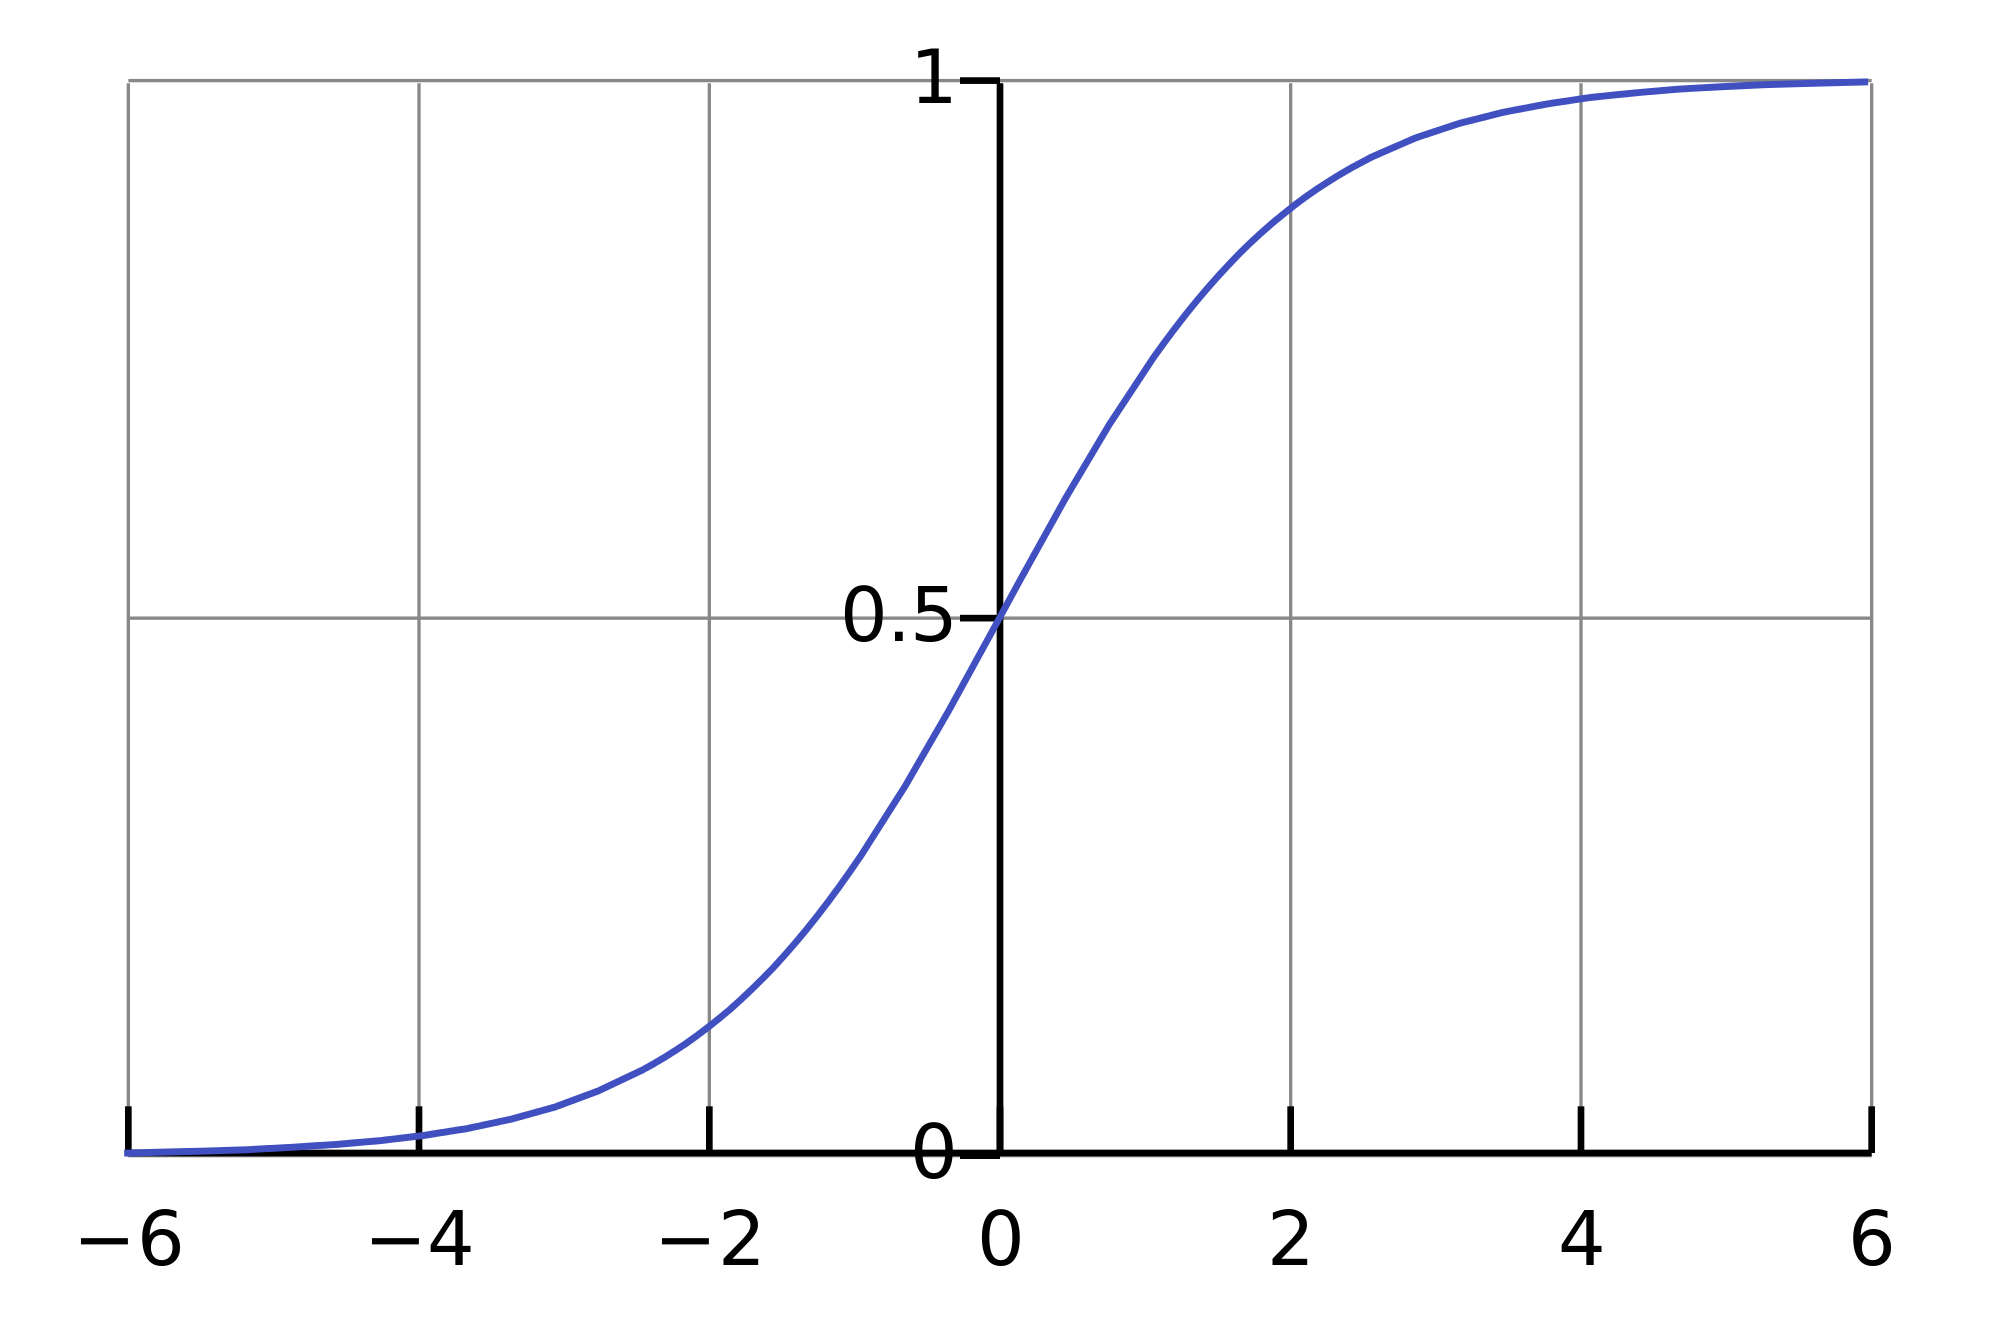
\includegraphics[width=3in]{fig/sigmoid}
  \caption{Graph of logistic (sigmoid) function}\label{fig:sigmoid}
\end{figure}

The logistic regression classifier uses the logistic function of the {\em weighed}
(as well as biased) sum of the input variables to predict the probability of
the input set belonging to a class (or category). The probability function is
already fixed. The only thing that we can change while learning from different
training set is the set of weight parameters ($\theta$) assigned to each feature.

\subsection{The Algorithm}

Let,
\begin{align}
  m &= \text{number of samples in training set}
  \nonumber\\
  n &= \text{number of features} \ge 1
  \nonumber\\
  x &= \text{input feature vector} =
  \begin{bmatrix}
  x_0 \\ x_1 \\ x_2 \\ \vdots \\ x_n
  \end{bmatrix}, x_0 = 1 \text{(always)}
  \nonumber\\
  y &= \text{class} \in \{ 1, 0 \} \text{ with 1 as primary class}
  \nonumber
\end{align}

The training set for this machine learning algorithm is the set of $m$ training
samples (examples).
\begin{align}
  \text{training set} = 
  \left\{ (x^{(1)}, y^{(1)}), (x^{(2)}, y^{(2)}), \cdots , (x^{(m)}, y^{(m)}) \right\}
  \label{eqn:training-set}
\end{align}

The weight parameters for the $(n+1)$ features are given by:
\begin{align}
  \theta = 
  \begin{bmatrix}
    \theta_0 \\ \theta_1 \\ \theta_2 \\ \vdots \\ \theta_n
  \end{bmatrix}
  \nonumber
\end{align}

Then the hypothesis function used to predict the output $y$ for
input feature set $x$ with parameter $\theta$ is given by:
\begin{align}
  \text{h}_{\theta}(x) = 
  \text{sigmoid}\left( \sum_{i = 0}^{n} \theta_{i} x_{i}\right) =
  \text{sigmoid}\left( \theta^{T}x \right) =
  \frac{1}{1 + e^{-\theta^{T}x}}
  \label{eqn:hypothesis}
\end{align}

Now the aim of this machine learning algorithms is to adjust the parameters
$\theta$ to fit the hypothesis $h_{\theta}(x)$ with the real output $y$ of
training set with minimum cost (error). For that, we need to define the cost
function, preferably, a {\em convex} cost function. There are different types
of cost functions. Linear regression, for instance, uses the sum of the squares
of the errors as the cost function. But in logistic regression, since the output
is not linear (even though the input is), this cost function turns out to be
non-convex and there are not efficient algorithms that can minimize a non-convex
function. Therefore, we define a logarithmic cost function $J(\theta)$ for logistic regression
as follows:
\begin{align}
  \text{J}(\theta) = \frac{1}{m} \sum_{i=1}^{m}
  \text{Cost} \left( \text{h}_\theta \left(x^{(i)} \right), y^{(i)} \right)
  \label{eqn:j}
\end{align}
where,
\begin{align}
  \text{Cost} (h, y) &=
  \begin{cases}
    -\log (h) &\text{ for } y = 1 \\
    -\log (1-h) &\text{ for } y = 0
  \end{cases}
  \nonumber\\
  &= -y\log(h) - (1-y)\log(1-h)
  \label{eqn:cost}
\end{align}

After we define an appropriate convex cost function J($\theta$), the machine
learning algorithm basically boils down to finding parameter $\theta$
that minimizes J($\theta$).
\begin{align}
  \min_{\theta} \quad \text{J}(\theta)
\end{align}

This can be achieved using varitous optimization algorithms. Some notable
ones are Gradient descent, BFGS, Quasi-Newton, L-BFGS, etc. The gradient
descent is the simplest one. It is a hill-climbing optimization algorithm
that tries finds the local optima from the start point. But since our
cost function J($\theta$) is convex, there is only one minima and that is the
global minima.

To find parameter $\theta$ that minimizes the cost function J($\theta$),
we initial $\theta$ with small random values and then
iterate the following until convergence:
\begin{align}
  \theta_j = \theta_j - \alpha \frac{\partial \text{J}(\theta)}{\partial \theta_j};
  \quad j \in {0,1,2,\ldots,n}; \quad \alpha = \text{learning rate}
  \nonumber
\end{align}
where,
\begin{align}
  \frac{\partial \text{J}(\theta)}{\partial \theta_j} =
  \sum_{i=1}^{m} \left( \text{h}_\theta \left(x^{(i)}\right) - y^{(i)} \right) x^{(i)}_j
\end{align}
Note that all $\theta_j$'s must be updated simultaneously. This concept is called
{\em batch learning}, contrary to {\em online learning} where the parameter is updated
separately for every training example.

The resulting parameter $\theta$ that minimizes the cost function J($\theta$) is
the parameter of the learning model. Then we can use the hypothesis $h_\theta(x)$
to predict the output $y$ for any input feature set $x$. The output $y$ will be
a value in the range $(0,1)$. The output can be interpreted as the probability
of the given input set belonging to the class 1 (primary class).

Other advanced optimization algorithms such as BFGS, L-BFGS, Quasi-Newton, etc.
are more efficient that the basic gradient descent and also has the advantage that
we don't have to manually select the learning rate ($\alpha$). These advanced
optimization algorithms will automatically select the appropriate value of $\alpha$
to maximize efficiency.

\subsection{Other Considerations}


\subsubsection{Feature Scaling}

Feature scaling is the process of scaling (or normalizing) all the features
to a limit of $[-1,1]$ or $[0,1]$. This is required because unscaled features
causes some features to get higher priority implicitly and it reduces
the accuracy of the learning algorithm. Feature scaling can be done in following
ways:
\begin{align}
  x_j^{(i)} &= \frac{x_j^{(i)} - \min (x_j)}{ \max (x_j) - \min (x_j)}
  \in [0, 1]
  \nonumber
\end{align}
or
\begin{align}
  x_j^{(i)} &= \frac{x_j^{(i)} - \overline{x_j}}{ \max (x_j) - \min (x_j)}
  \in [-1, 1]
  \nonumber
\end{align}
or
\begin{align}
  x_j^{(i)} &= \frac{x_j^{(i)} - \overline{x_j}}{\sigma_{x_j}}
  \quad (\text{for normal distribution})
  \nonumber
\end{align}


\subsubsection{Regularization}

Regularization is the process of scaling down the values of parameter $\theta$
to reduce the problem of over-fitting. Over-fitting is the condition when
the learning algorithm satisfies the training set very precisely but doesn't
satisfy test data (not included in training set). Regularization is done
by introducing a regularization parameter $\lambda$ term in the overall
cost function J($\theta$).
\begin{align}
  \text{J}(\theta) = \frac{1}{m} \sum_{i=1}^{m}
  \text{Cost} \left( \text{h}_\theta \left(x^{(i)} \right), y^{(i)} \right)
  + \frac{\lambda}{2m} \sum_{j=0}^n \theta_j^2
  \label{eqn:j-with-l}
\end{align}
The corresponding first-order derivatives then becomes:
\begin{align}
  \frac{\partial \text{J}(\theta)}{\partial \theta_j} &=
  \begin{cases}
    \displaystyle
    \sum_{i=1}^{m} \left( \text{h}_\theta \left(x^{(i)}\right) - y^{(i)} \right) x^{(i)}_j
    &\text{ for } j = 0\\
    \displaystyle
    \sum_{i=1}^{m} \left( \text{h}_\theta \left(x^{(i)}\right) - y^{(i)} \right) x^{(i)}_j
    + \frac{\lambda}{m} \theta_j
    &\text{ for } j \in {1,2,\ldots,n}
  \end{cases}
  \nonumber
\end{align}
